\documentclass{standalone}

\usepackage[utf8]{inputenc}

% Page setup
\usepackage{amsmath}

% Typography
\usepackage[scaled]{helvet}
\let\familydefault\sfdefault

\usepackage[usenames,svgnames]{xcolor}
\usepackage{tikz,pgfplots}
\usetikzlibrary{positioning,arrows,intersections,calc}

\definecolor{colorinput}    {RGB}{199,212,104}
\definecolor{colormodule}   {RGB}{ 79,142,209}

\begin{document}
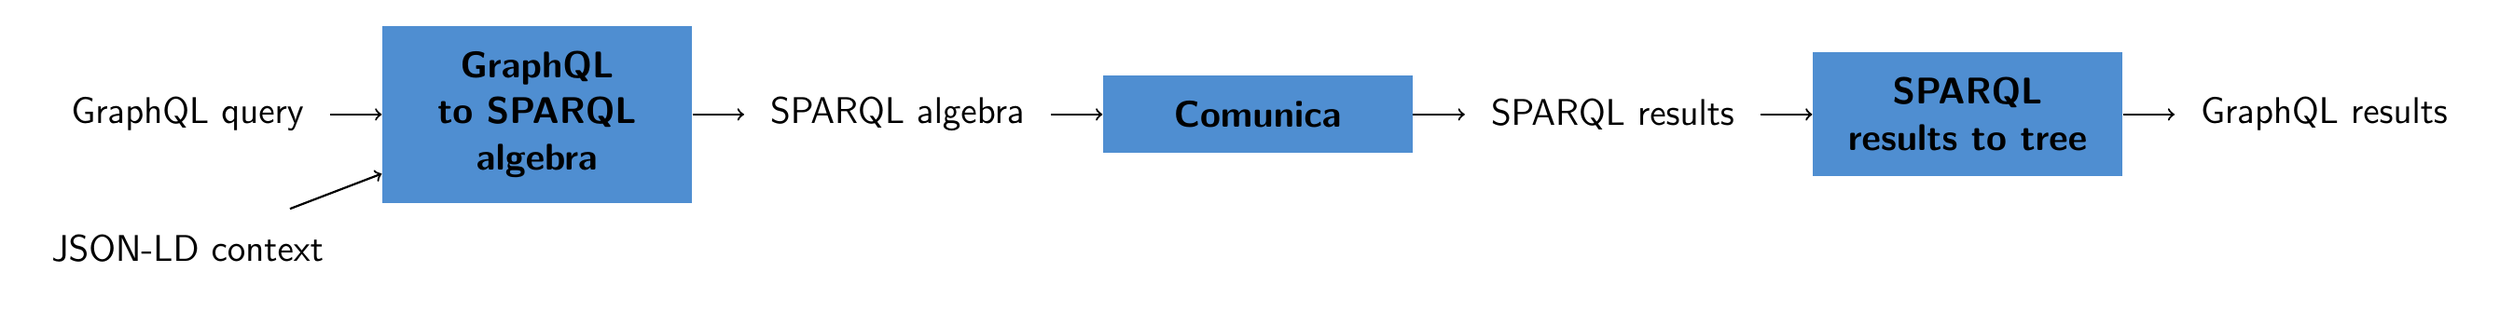
\begin{tikzpicture}[
    node distance = 2em, auto,
    font={\Large\itshape},
    base/.style={font={\Large\bfseries},inner sep=10pt,align=center,rectangle},
    baseinput/.style={font={\Large},inner sep=10pt,align=center,rectangle},
]

    \node[baseinput]                (query)   {GraphQL query};
    \node[baseinput,below=of query] (context) {JSON-LD context};
    
    \node[base,fill=colormodule,text width=10em,right=of query](parser)  {GraphQL to SPARQL algebra};
    
    \node[baseinput,right=of parser](algebra)  {SPARQL algebra};
    
    \node[base,fill=colormodule,text width=10em,right=of algebra](comunica)  {Comunica};
    
    \node[baseinput,right=of comunica](results)  {SPARQL results};
    
    \node[base,fill=colormodule,text width=10em,right=of results](shaper)  {SPARQL results to tree};
    
    \node[baseinput,right=of shaper](graphqlresults)  {GraphQL results};
    
    \draw[->,thick](query) -- (parser);
    \draw[->,thick](context) -- (parser);
    
    \draw[->,thick](parser) -- (algebra);
    
    \draw[->,thick](algebra) -- (comunica);
    
    \draw[->,thick](comunica) -- (results);
    
    \draw[->,thick](results) -- (shaper);
    
    \draw[->,thick](shaper) -- (graphqlresults);

\end{tikzpicture}
\end{document}
